\section{Anexo 1, Manual de usuario}
En el siguiente anexo se presenta el manual de usuario del proyecto,
el cual contiene las instrucciones necesarias para la instalación y
ejecución del mismo. Además, se incluye una guía de uso con el que
poder continuar el desarrollo del proyecto en caso de ser necesario.

\subsection{Instalación}
Para la instalación del proyecto se requiere de un sistema operativo
Linux que tenga instalado una versión de Python 3.10 o superior. En
el desarrollo se ha utilizado Pyenv para la gestión de versiones de
Python, pero no es estrictamente necesario para la instalación del 
proyecto.\medskip

El primer paso es clonar el repositorio del proyecto, para ello es
necesario tener instalado Git en el sistema. Una vez clonado el
repositorio, ejecutaremos el comando \textit{Make install} para 
instalar las dependencias del proyecto y crear el entorno virtual
de Python. Esto nos proporcionara una instalación básica del proyecto
para el entrenamiento y desarrollo de los modelos. Además, adicionalmente
se instalará la última versión de pre-commit para la gestión de los
estilos de código.

\subsection{Ejecución del proyecto}
El proyecto cuenta con diferentes comandos para la ejecución de los
diferentes procesos que se pueden realizar. Para la ejecución de los
comandos se utiliza el comando \textit{Make}, seguido del nombre del
comando que se desea ejecutar. A continuación se detallan los comandos
disponibles en el proyecto:
\begin{itemize}
    \item \textbf{Make install.} Instala las dependencias básicas del proyecto,
    pre-commit y crea el entorno virtual de Python.
    \item \textbf{Make train.} Inicia el entrenamiento del modelo, una vez
    finalizado el entrenamiento se guardará el modelo en la carpeta
    \item \textbf{Make eval.} Inicia la evaluación del modelo, este comando
    utiliza el benchmark situado en el archivo \textit{data/benchmark} que
    contiene las instancias junto con la mejor solución para cada una de ellas.
    \textit{models} del proyecto. Para la ejecución de este comando es
    necesario generar el dataset de entrenamiento y validación.
    \item \textbf{Make optimization.} Inicia el proceso de optimización
    de hiperparámetros del modelo. Para la ejecución de este comando es
    necesario generar el dataset de entrenamiento y validación.
    \item \textbf{Make gen-train gen-val.} Genera el dataset de entrenamiento
    y validación respectivamente.
    \item \textbf{Make sync.} Sincroniza las dependencias del proyecto con
    el fichero \textit{requirements.txt.} Este comando es necesario para
    los casos en los que se añadan nuevas dependencias al proyecto.
    \item \textbf{Make compile.} Compila el proyecto para la generación de
    dependencias de forma automática.
    \item \textbf{Make test.} Lanza los test del proyecto.
    \item \textbf{Make clean.} Elimina los ficheros generados por el proyecto.
\end{itemize}

\subsection{Visualización de resultados}
La visualización de los resultados se realiza mediante el uso de una interfaz 
gráfica desarrollada con Streamlit como se ha comentado anteriormente. 
Debido a que la visualización es un añadido al proyecto, las dependencias 
necesarias para su ejecución no se instalan de forma automática ya que no 
son necesarias para el entrenamiento y algunas de ellas presentan incompatibilidades
con otras que si son imprescindibles. Para su instalación ejecutaremos el
comando \textit{Make install-app} y en caso de querer volver al estado 
anterior podremos ejecutar \textit{Make sync}.\medskip

Una vez instaladas las dependencias, para la ejecución de la aplicación
ejecutaremos el comando \textit{Make app} y se abrirá una ventana en el
navegador con la aplicación. En caso de que no se abra automáticamente,
podremos acceder a la aplicación mediante la dirección \textit{localhost:8501}.

\begin{figure}[ht]
    \centering
    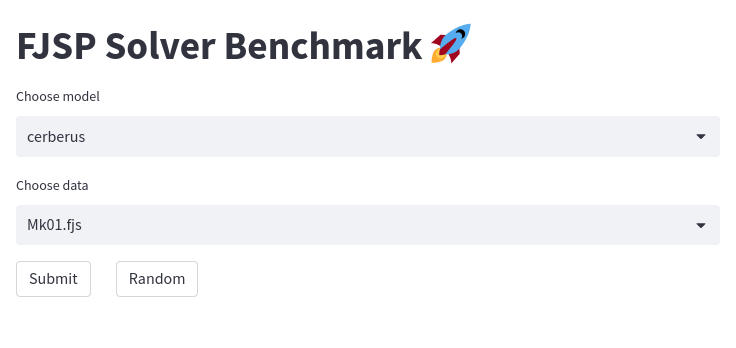
\includegraphics[width=\textwidth]{base-app.png}
    \caption{Pagina principal de la aplicación.}
    \label{fig:demo}
\end{figure}

Esta aplicación permite visualizar los resultados de los diferentes
benchmark que se han realizado durante el desarrollo del proyecto. En la
figura \ref{fig:demo} se puede ver la página principal de la aplicación,
en la que se muestra un desplegable con los diferentes benchmarks que se
pueden visualizar. Una vez seleccionado el benchmark y pulsado el botón
\textit{Submit}, se mostrará un Gantt con los resultados de las diferentes
tareas asignadas a cada máquina. A continuación, se muestra un ejemplo de
la visualización de un benchmark.

\begin{figure}[ht]
    \centering
    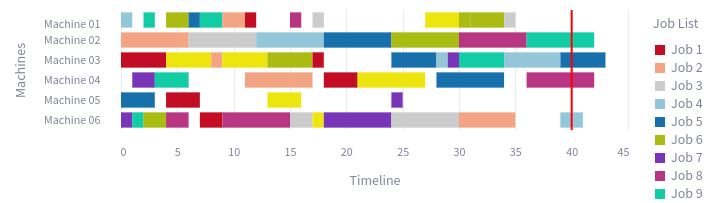
\includegraphics[width=0.8\textwidth]{jobgantt.png}
    \caption{Visualización del Gantt de tareas.}
    \label{fig:demo-2}
\end{figure}

\pagebreak
